\section{Display}

\subsection{LCD-kredsløb}
%%%%%BILLEDE AF KREDSLØB
\begin{figure}[H]
	\centering
    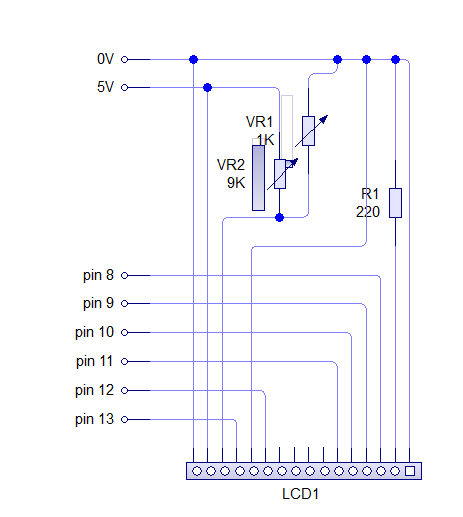
\includegraphics[height=10cm]{/circuit/LCDkreds.PNG}
	\caption{Arduino LCD kreds lavet ud fra arduino siden, se \cite{arduinoLCD}}
	\label{arduinoLCD}
\end{figure}
\subsubsection{LCD setup}
Vi benytter et LCD display, da det let kan forbindes direkte til arduioen uden et ekstra interface ved brug af LiquidCrystal biblioteket. Biblioteket vi benytter gør brug af ASCII kode se figur ~\ref{ASCII} til at vise symboler på et display.
Vi benyttede et 4-bit datainterface setup (se \cite{arduinoLCD}), hvor displayet skriver på to linjer.




% Skriv om teori. Skriv om 4-bit interface
\subsection{Teori}
\subsubsection{LiquidCrystal library}
LiquidCrystal library bruger vi til at kunne få arduinoen til at sende den ønskede tekst af f.eks. af en måling til et LCD. LiquidCrystal gør brug af ASCII kode til at tolke binære signaler til tekst se Figur ~\ref{ASCII}
\begin{figure}[H]
	\centering
    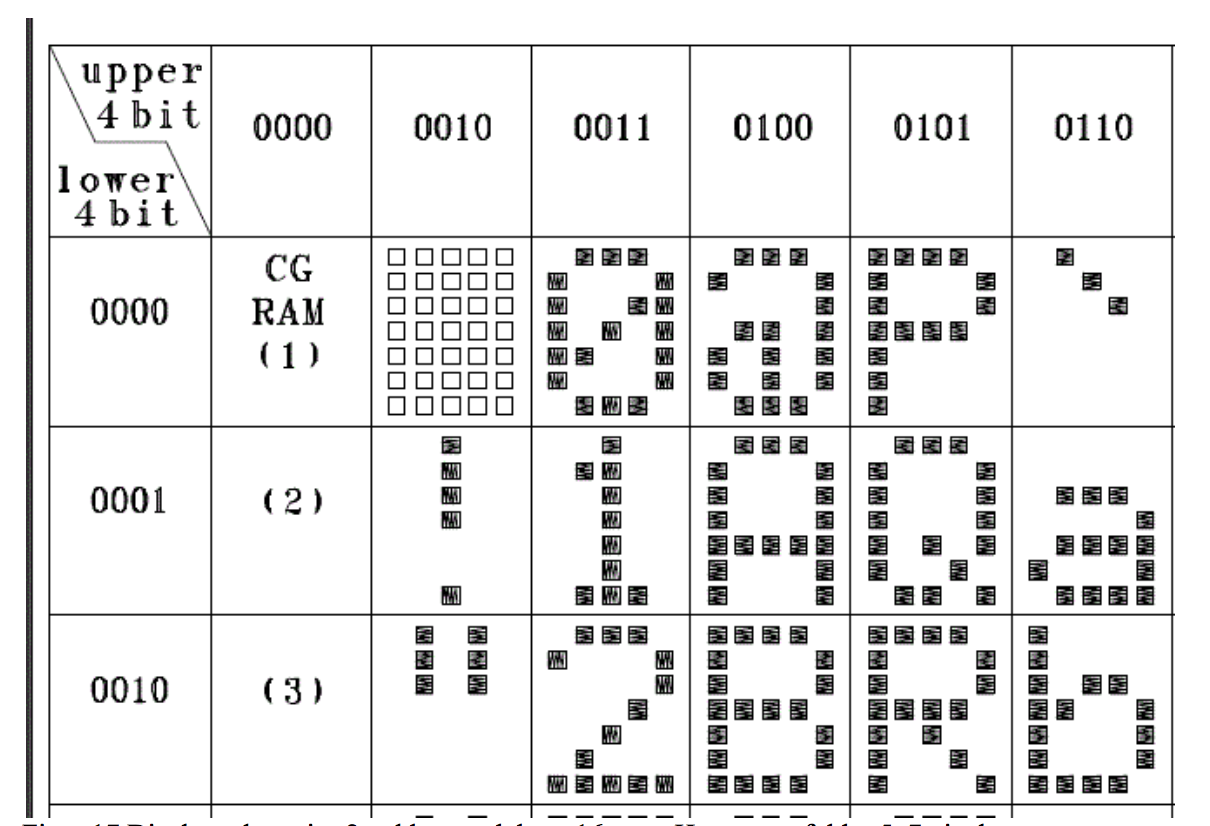
\includegraphics[width=10cm]{/LCDdesign/ASCII.png}
	\caption{Et eksempel på nogle ASCII koder benyttet af LiquidCrystal library - kilde: [Uddrag fra projektvejledning]}
	\label{ASCII}
\end{figure}
\subsection{Komponenter}
\subsubsection{Arduino}
Se afsnit \ref{sec:arduino} 
% ************** kilde

% Skriv om displayet og displaydriveren
\subsubsection{LCD display}
LCD displayet vi benyttede havde en indbygget controller som vist på Figur ~\ref{driver}.
\begin{figure}[H]
	\centering
    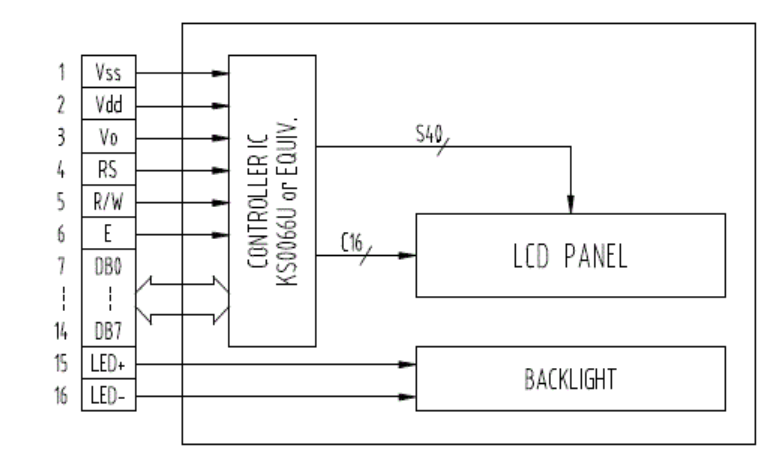
\includegraphics[width=10cm]{/LCDdesign/displayblokdiagram.png}
	\caption{Et blok diagram over databen og kontrolben til  kontroller, backlight, LCD panel. Kontrolleren er indbygget i displayet. kilde: [Uddrag fra projektvejledning]}
	\label{driver}
\end{figure}


 
\subsection{Test}
Vi benyttede en simpel "Hello World" program til at teste skærmen, koden fik vi fra \cite{arduinoLCD}.





% Begin CODE EXAMPLE
% ---------------------------
\begin{lstlisting}[caption=kodeeksempel "Hello World" med timer, label={alg:helloworld}]
// Inkluder koden fra liquidcrystal library:
#include <LiquidCrystal.h>

//Initialiser biblioteket 
//med disse interfacepins.
LiquidCrystal lcd(12, 11, 5, 4, 3, 2);

void setup() {
//Bestemmer antallet af hhv.
//kolonner og rækker for displayet
  lcd.begin(16, 2);
//Printer besked til displayet
  lcd.print("hello, world!");
}

void loop() {
// Sætter cursor til at være på anden række,
// som er markeret 1.
  lcd.setCursor(0, 1);
//Printer antallet af sekunder der 
//er gået siden reset.
  lcd.print(millis() / 1000);
}
\end{lstlisting}
% ----------------------------------
% End code example


Potentiometret kunne justerer skærmens styrke fint.
\begin{figure}[H]
	\centering
    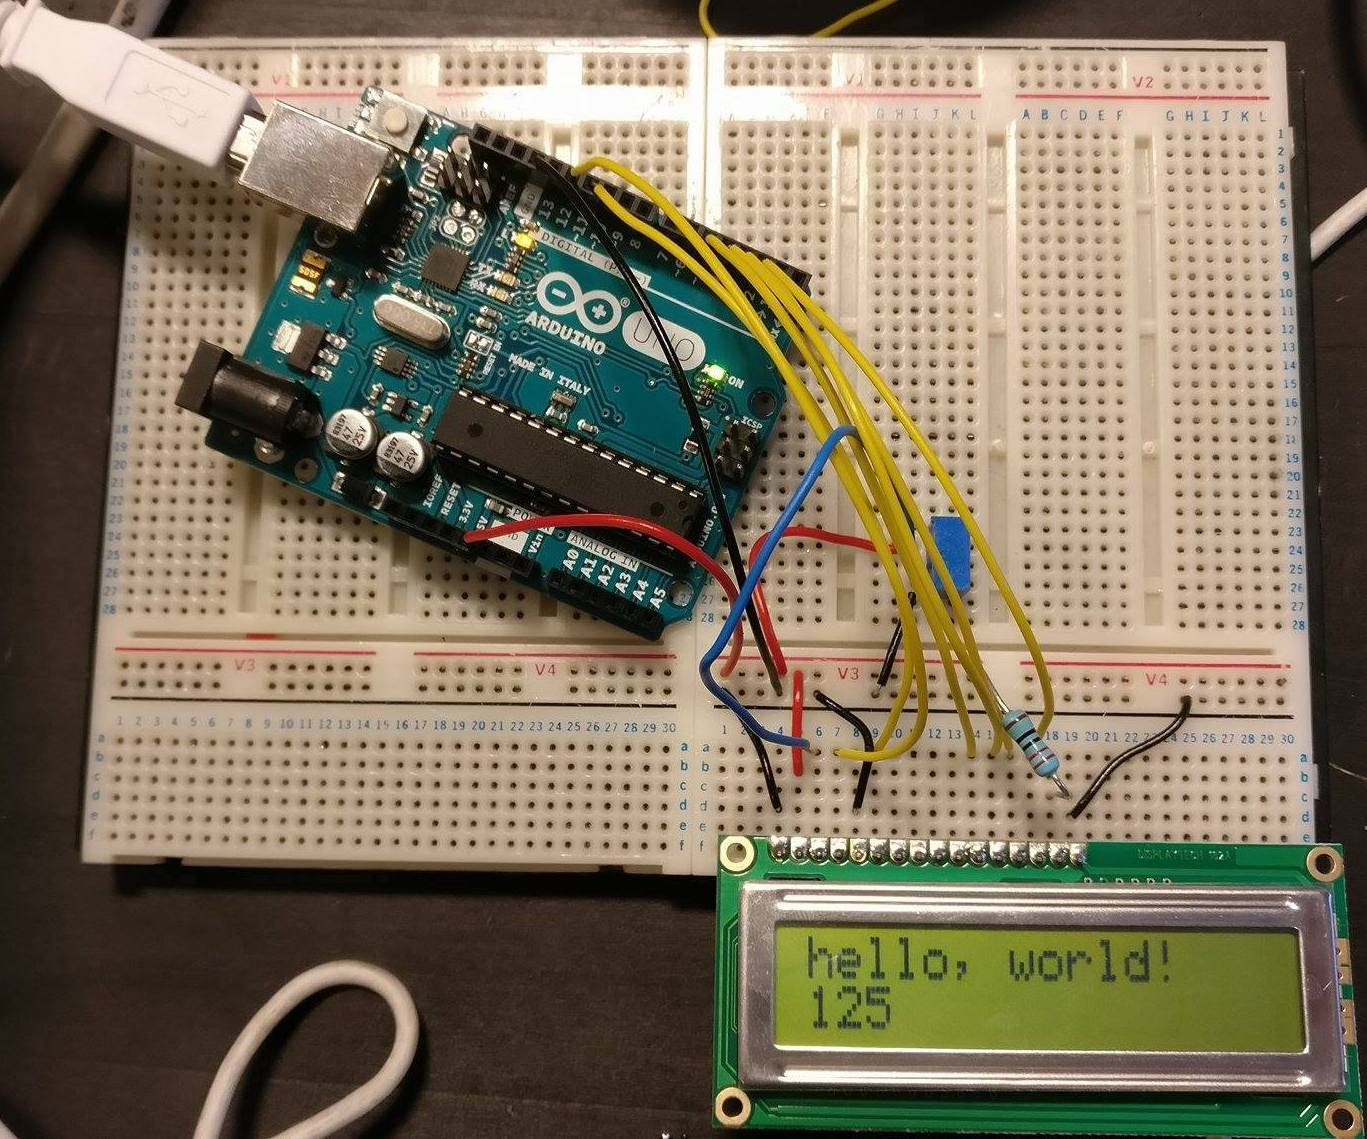
\includegraphics[width=10cm]{/LCDdesign/Displaykreds}
	\caption{Dokumentation af vores LCD sluttet til arduinoen, der benyttes Kode \ref{alg:helloworld}}
	\label{fig: dispalykreds}
\end{figure}
